% !Mode::"TeX:UTF-8"

% -------------------- Information --------------------

\newcommand{\TITLE}{有限差分方法}
\newcommand{\AUTHOR}{Jason}
\newcommand{\SUBJECT}{偏微分方程数值解}
\newcommand{\KEYWORDS}{}

% -------------------- Packages --------------------

\documentclass[a4paper, 12pt]{ctexart}
\usepackage{amsmath}
\usepackage{amssymb}
% \usepackage{amsthm} % 定理格式 由ntheorem代替.
\usepackage{authblk} % 作者 (见校赛论文).
\usepackage{array}
\usepackage{bigfoot} % to allow verbatim in footnote.
\usepackage{bm} % \bm for bold symbols.
\usepackage{boldline} % 长表格表格线加粗.
\usepackage{caption} % 题注.
\usepackage{commath} % abs, norm
\usepackage{enumerate}
% \usepackage{enumitem} 用enumerate包代替.
\usepackage{fancyhdr} % 脚注.
\usepackage{filecontents}
\usepackage{flafter} % 不让float出现在定义之前的地方.
\usepackage{float} % 你们这帮float给我乖乖听话 HHHHHHHHHHH.
\usepackage[T1]{fontenc} % Bera Mono Font
\usepackage{fontspec} % 字体.
\usepackage{graphicx}
\usepackage{hyperref}
\usepackage{lastpage}
\usepackage{letltxmacro} % \let
\usepackage{lipsum}
\usepackage{listings} % 排版程序语言.
\usepackage{longtable} % 长表格.
\usepackage{makecell} % 表格线加粗 \Xhline{1.2pt}.
\usepackage{mathtools} % \xleftrightarrow.
\usepackage{mathrsfs} % \mathscr
\usepackage{multirow} % 合并单元格.
\usepackage[square, numbers, sort&compress]{natbib} % 引用.
\usepackage[thmmarks, amsmath, thref]{ntheorem} % 定理格式.
\usepackage[section]{placeins} % 使图像不会显示在别的部分 若过于严格则换成[below].
\usepackage{stackrel} % 上下写 见校赛论文.
\usepackage{subcaption} % subcaption and subfigure
% \usepackage{SUBSubsubsection}
\usepackage{titlesec} % Section标题格式.
\usepackage{varioref} % For Cross References.
\usepackage[dvipsnames]{xcolor} % 颜色声明.
\usepackage{xfrac} %\sfrac{}{}
\usepackage[all, cmtip]{xy} % Commutive diagram.

% Require `ntheorem'

\usepackage[mathlines, edtable]{lineno} % Line numbers.
    %\begin{edtable}{tabular}[<args>] <entries> \end{edtable}

% Require `xcolor'

\usepackage[numbered, framed]{matlab-prettifier}
\usepackage{pgfplots}
\usepackage{pgfplotstable}
\usepackage{tikz}

% Incompatible with `matlab-prettifier'

\usepackage[printwatermark]{xwatermark} % Foreground Watermarks.

% -------------------- Settings --------------------

% Title

\title{\TITLE}
\author{\AUTHOR}
\date{\today}

% Package: caption

\captionsetup{
    margin    =   6pt,
    font      =   small,
    labelfont =   bf
}

% Package: ctex

\setCJKfamilyfont{fzstk}{FZShuTi} % 方正舒体
\newcommand{\fzstk}{\CJKfamily{fzstk}}

% Package: fancyhdr

\setlength{\headheight}{15pt}
\lhead{Copyright \copyright\ \AUTHOR}
\rhead{Page \thepage\ of \pageref{LastPage}}

% Package: graphicx

\graphicspath{{resources/}} % 图像文件目录

% Package: hyperref

\hypersetup{
    linktoc             =   all,
    colorlinks          =   true,
    linkcolor           =   cyan,
    anchorcolor         =   black,
    citecolor           =   green,
    filecolor           =   cyan,
    menucolor           =   red,
    runcolor            =   filecolor,
    urlcolor            =   magenta,
	pdftitle           	=   {\TITLE},
	pdfauthor          	=   {\AUTHOR},
	pdfsubject         	=   {\SUBJECT},
	pdfcreator			=	{Visual Studio Code},
	pdfproducer			=	{XeLaTeX with documentclass ctexart},
	pdfkeywords        	=   {\KEYWORDS},
    bookmarksnumbered   =   true,
    pdfstartview        =   FitH,
    pdfpagelayout       =   OneColumn
}

% Package: lineno

\renewcommand{\linenumberfont}{\normalfont\scriptsize\sffamily}

\let\oldlstinputlisting\lstinputlisting
\renewcommand{\lstinputlisting}[2][\empty]{
    \par\nolinenumbers\oldlstinputlisting[#1]{#2}\linenumbers\par
}

\let\oldlstlisting\lstlisting
\let\oldendlstlisting\endlstlisting
\renewenvironment{lstlisting}
    {\par\nolinenumbers\oldlstlisting}
    {\oldendlstlisting\endnolinenumbers\par}

\let\oldtable\table
\let\oldendtable\endtable
\renewenvironment{table}
    {\par\nolinenumbers\oldtable}
    {\oldendtable\endnolinenumbers\par}

% Package: listings

%% Title

\renewcommand\lstlistingname{代码}
\renewcommand\lstlistlistingname{代码}

%% Lstinline with color box

\LetLtxMacro{\oldlstinline}{\lstinline}
\renewcommand{\lstinline}[2][]{\colorbox{lightgray}{\oldlstinline[#1]{#2}}}
\newcommand{\matlabinline}[1]{
    \lstinline[style=MATLAB-editor, basicstyle=\mlttfamily]{#1}}

\lstset{
    breaklines=true,
    backgroundcolor=\color{lightgray},
    basicstyle=\scriptsize,
    inputpath=resources/,
    numbers=left,
    numberstyle={\color{black!33}\scriptsize\sffamily},
    xleftmargin=2em,
    xrightmargin=2em
}

% Package: ntheorem

%% Theorem
\newtheorem{theorem}{Theorem}[section]
\newtheorem{lemma}[theorem]{Lemma}
\newtheorem{corollary}[theorem]{Corollary}
%% Problem
\theoremstyle{plain}
\newtheorem{problem}{Problem}[section]
%% Proposition
\newtheorem{proposition}{Proposition}[section]
%% Conjecture
\newtheorem{conjecture}[proposition]{Conjecture}
%% Definition
\theoremstyle{plain}
\theoremheaderfont{\bfseries}
\theorembodyfont{\rmfamily}
\newtheorem{definition}{Definition}[section]
%% Note
\theoremstyle{plain}
\theoremheaderfont{\itshape}
\theorembodyfont{\itshape}
\newtheorem{note}{Note}[section]
%% Proof
\theoremstyle{nonumberplain}
\theoremheaderfont{\itshape}
\theorembodyfont{\upshape}
\theoremseparator{.}
\theoremsymbol{\ensuremath{\square}}
\newtheorem{proof}{Proof}
%% Solution
\theoremsymbol{\ensuremath{\blacksquare}}
\newtheorem{solution}{Solution}

% Package: pgfplots

\pgfplotsset{width=7cm, compat=1.16}

% Package: pgfplotstable

\pgfplotstableset{
    every head row/.style={before row=\Xhline{1.2pt},after row=\hline},
    every last row/.style={after row=\Xhline{1.2pt}}
}

% Package: varioref

\renewcommand{\reftextbefore}
    {on the \reftextvario{preceding page}{page before}}
\renewcommand{\reftextafter}
    {on the \reftextvario{following}{next} page}
\renewcommand{\reftextfacebefore}
    {on the \reftextvario{facing}{preceding} page}
\renewcommand{\reftextfaceafter}
    {on the \reftextvario{facing}{next} page}
\renewcommand{\reftextfaraway}[1]
    {on page \pageref{#1}}

%% Label formats

\labelformat{lstlisting}{代码#1}
\labelformat{equation}{式(#1)}
\labelformat{figure}{图#1}
\labelformat{table}{表#1}
\labelformat{problem}{Problem #1}

% Package: xwatermark

\newsavebox\mybox
\savebox\mybox{\tikz[color=cyan, opacity=0.2]\node{\fzstk\SUBJECT};}
\newwatermark*[
    allpages,
    angle=45,
    scale=6,
    xpos=-20,
    ypos=15
]{\usebox\mybox}

% -------------------- General new commands --------------------

\DeclareMathAlphabet{\mathsfsl}{OT1}{cmss}{m}{sl}

\DeclareMathOperator{\arcosh}{arcosh}
\DeclareMathOperator{\Arcosh}{Arcosh}
\DeclareMathOperator*{\Beta}{B}
\DeclareMathOperator{\Log}{Log}
\DeclareMathOperator*{\real}{Re}
\DeclareMathOperator*{\image}{Im}

% Expectation

\newcommand{\expect}{\operatorname{E}\expectarg}
\DeclarePairedDelimiterX{\expectarg}[1]{(}{)}{
    \ifnum\currentgrouptype=16 \else\begingroup\fi
    \activatebar#1
    \ifnum\currentgrouptype=16 \else\endgroup\fi
}

\newcommand{\innermid}{\nonscript\;\delimsize\vert\nonscript\;}
\newcommand{\activatebar}{
    \begingroup\lccode`\~=`\|
    \lowercase{\endgroup\let~}\innermid
    \mathcode`|=\string"8000
}

\newcommand*{\BC}{\mathbb{C}}
\newcommand*{\BR}{\mathbb{R}}
\newcommand*{\diff}{\mathop{}\!\mathrm{d}}
\newcommand*{\matr}[1]{\ensuremath{\mathsfsl{#1}}} % italic sans serif
\newcommand*{\me}{\mathrm{e}}
\newcommand*{\mi}{\mathrm{i}}
\newcommand*{\restrict}[1]{\raisebox{-.5ex}{$\vert$}_{#1}}
\newcommand*{\vect}[1]{\bm{#1}}

% -------------------- Specific new commands --------------------



% -------------------- Document --------------------

\begin{document}

    % -------------------- Title Page --------------------

    \maketitle
    \thispagestyle{empty}
    \pagenumbering{roman}

    % -------------------- Abstract Page --------------------

    % -------------------- Contents --------------------

    \newpage
    \tableofcontents

    % -------------------- Body --------------------

    \newpage
    \pagestyle{fancy}
    \pagenumbering{arabic}
    \linenumbers

    \section{知识点}

    若有二阶线性常微分方程
    \begin{equation}
        -\frac{\diff}{\diff x}\left(p\frac{\diff u}{\diff x}\right)+qu=f,\quad x\in(a,b),
    \end{equation}
    用步长$h$离散区域和微分方程, 可得方程组
    \begin{equation}
        -\frac{1}{h}\left(p_{i+\frac{1}{2}}\frac{u_{i+1}-u_{i}}{h}-p_{i-\frac{1}{2}}\frac{u_{i}-u_{i-1}}{h}\right)+q_{i}u_{i}=f_{i},\quad i=1,2,\dotsc,N-1.
    \end{equation}

    \section{练习题}

    \begin{problem}
        \label{problem: 1}
        利用有限差分方法求解如下常微分方程边值问题:
        \begin{equation}
            \left\{
            \begin{aligned}
                &\frac{\diff^{2}T}{\diff x^{2}}-0.15T=0,\quad x\in [0, 10],\\
                &T(0)=240,\quad T(10)=150.
            \end{aligned}
            \right.
        \end{equation}
    \end{problem}

    \begin{solution}
        我们将分别求出真解与数值解.
        
        利用Sturm-Liouville边值问题的相关知识可求出真解
        \begin{equation}
            T(x) = C_{1}\me^{\sqrt{0.15}x}+C_{2}\me^{-\sqrt{0.15}x},
        \end{equation}
        其中
        \begin{equation}
            C_{1} = \frac{150-240\me^{-\sqrt{15}}}{\me^{\sqrt{15}}-\me^{-\sqrt{15}}},
            \quad
            C_{2} = \frac{240\me^{\sqrt{15}}-150}{\me^{\sqrt{15}}-\me^{-\sqrt{15}}}.
        \end{equation}
        
        又本题中, $p(x)=-1$, $q(x)=-0.15$, $f(x)=0$. 设步长为$h$, 离散化区域和微分方程并代入边界条件, 可得方程组
        \begin{equation}
            \left\{
            \begin{aligned}
                &\frac{1}{h^{2}}T_{i-1}-\left(\frac{2}{h^{2}}+0.15\right)T_{i}+\frac{1}{h^{2}}T_{i+1}=0,\quad i=1,\dotsc,N-1,\\
                &T_{0}=240,\quad T_{N}=150.
            \end{aligned}
            \right.
        \end{equation}
        整理得$\matr{A}\vect{T}=\vect{b}$, 其中$\vect{T}=(T_{0},\dotsc,T_{N})^{T}$, $\vect{b}=(240, 0, \dotsc, 0, 150)^{T}$,
        \begin{equation}
            \matr{A}=
            \begin{pmatrix}
                1\\
                h^{-2} & -2h^{-2}-0.15 & h^{-2}\\
                & h^{-2} & -2h^{-2}-0.15 & h^{-2}\\
                & & \ddots & \ddots & \ddots\\
                & & & h^{-2} & -2h^{-2}-0.15 & h^{-2}\\
                & & & & & 1
            \end{pmatrix}
        \end{equation}

        选取不同的$N=1/h$进行计算, 得到图像:
        \begin{figure}[H]
            \centering
            \begin{subfigure}[b]{0.45\textwidth}
                \centering
                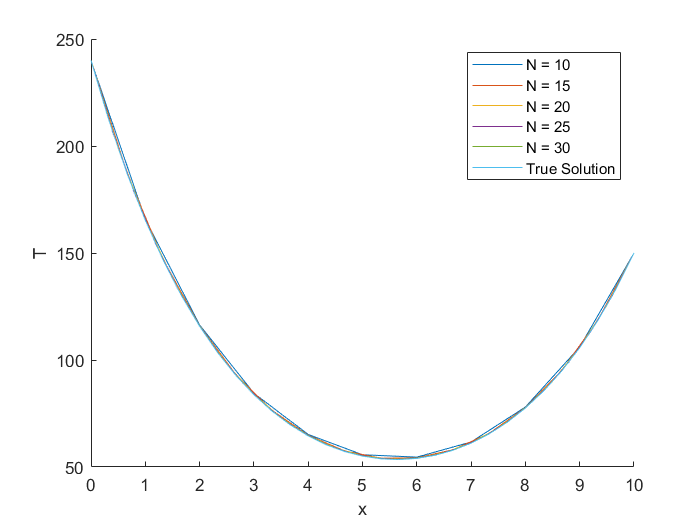
\includegraphics[width=\textwidth]{wc11.png}
                \caption{真解与数值解}
            \end{subfigure}
            \hfill
            \begin{subfigure}[b]{0.45\textwidth}
                \centering
                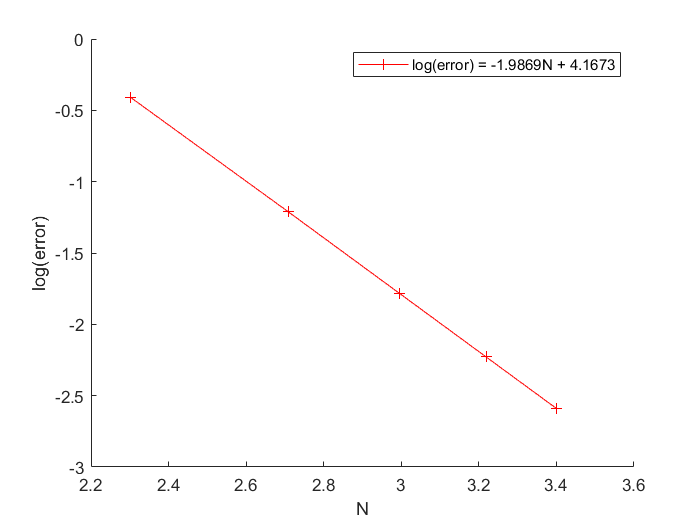
\includegraphics[width=\textwidth]{wc12.png}
                \caption{收敛阶}
            \end{subfigure}
            \caption{\ref{problem: 1}图像}
       \end{figure}

        可以看出约为2阶收敛.
    \end{solution}

    \begin{note}
        提一下本题中犯的错误好了. 当时写的追赶法mychase.m函数返回的向量是行向量, 而fdm.m函数返回的是列向量, 于是在执行
        \begin{lstlisting}[
            caption=去世现场,
            style=MATLAB-editor,
            basicstyle=\mlttfamily\scriptsize,
            numberstyle={\color{black!33}\scriptsize\sffamily}
        ]
error(i) = norm(T - sol(x), 'inf');
        \end{lstlisting}
        的时候就去世了, 而且还不会报错, 这直接导致了收敛阶曲线的斜率变成了正的.
    \end{note}

    \begin{problem}
        \label{problem: 2}
        利用有限差分方法求解如下常微分方程边值问题:
        \begin{equation}
            \left\{
            \begin{aligned}
                &7\frac{\diff^{2}y}{\diff x^{2}}-2\frac{\diff y}{\diff x}-y+x=0,\quad x\in [0, 20],\\
                &y(0)=5,\quad y(20)=8.
            \end{aligned}
            \right.
        \end{equation}
    \end{problem}

    \begin{solution}
        我们将分别求出真解与数值解.

        运用高阶常系数线性非齐次微分方程的求解方法, 先解出通解为
        \begin{equation}
            y = C_{1}\me^{(1+2\sqrt{2})x/7}+C_{2}\me^{(1-2\sqrt{2})x/7}+x-2.
        \end{equation}
        再代入边值条件求解常数$C_{1}$和$C_{2}$, 得
        \begin{equation}
            C_{1}=-\frac{7\me^{(20-40\sqrt{2})/7}+10}{\me^{(20+40\sqrt{2})/7}-\me^{(20-40\sqrt{2})/7}},
            \quad
            C_{2}=\frac{7\me^{(20-40\sqrt{2})/7}+10}{\me^{(20+40\sqrt{2})/7}-\me^{(20-40\sqrt{2})/7}}.
        \end{equation}

        又本题中, $p(x)=-7$, $q(x)=-1$, $f(x)=-x$. 设步长为$h$, 离散化区域和微分方程, 其中用三点公式近似代替导数$y'$, 代入边界条件, 可得方程组
        \begin{equation}
            \left\{
            \begin{aligned}
                &\left(\frac{7}{h^{2}}+\frac{1}{h}\right)y_{i-1}-\left(\frac{14}{h^{2}}+1\right)y_{i}+\left(\frac{7}{h^{2}}-\frac{1}{h}\right)y_{i+1}=-x_{i},\,i=1,\dotsc,N-1,\\
                &y_{0}=5,\quad y_{N}=8.
            \end{aligned}
            \right.
        \end{equation}
        整理得$\matr{A}\vect{y}=\vect{b}$, 其中$\vect{y}=(y_{0},\dotsc,y_{N})^{T}$, $\vect{b}=(5, -x_{1}, \dotsc, -x_{N-1}, 8)^{T}$,
        \begin{equation}
            \matr{A}=
            \begin{pmatrix}
                1\\
                7h^{-2} + h^{-1} & -14h^{-2}-1 & 7h^{-2} - h^{-1}\\
                & \ddots & \ddots & \ddots\\
                & & 7h^{-2} + h^{-1} & -14h^{-2}-1 & 7h^{-2} - h^{-1}\\
                & & & & 1
            \end{pmatrix}
        \end{equation}

        选取不同的$N=1/h$进行计算, 得到图像:
        \begin{figure}[H]
            \centering
            \begin{subfigure}[b]{0.45\textwidth}
                \centering
                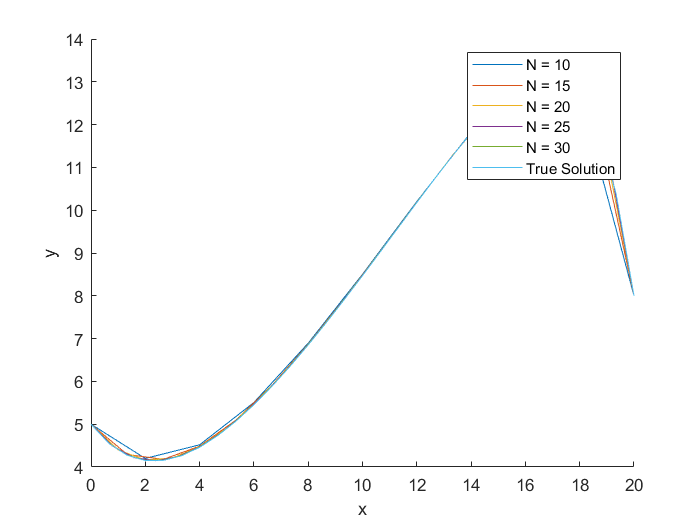
\includegraphics[width=\textwidth]{wc21.png}
                \caption{真解与数值解}
            \end{subfigure}
            \hfill
            \begin{subfigure}[b]{0.45\textwidth}
                \centering
                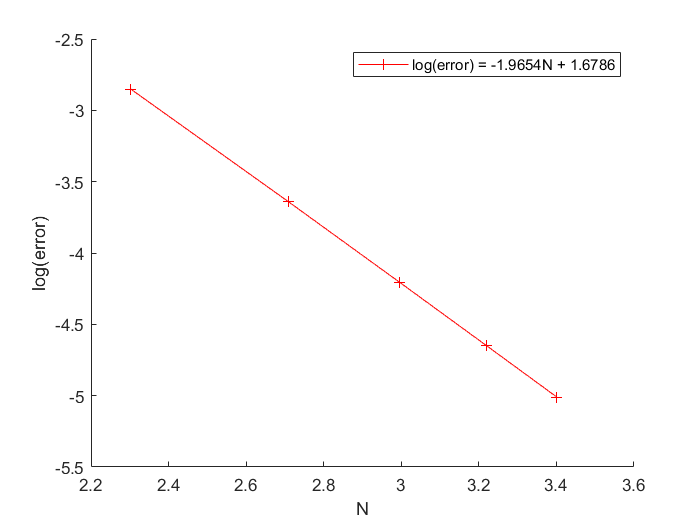
\includegraphics[width=\textwidth]{wc22.png}
                \caption{收敛阶}
            \end{subfigure}
            \caption{\ref{problem: 2}图像}
       \end{figure}

       可以看出约为2阶收敛.
    \end{solution}

    \begin{note}
        本题中我们也曾犯了一个低级错误, 漏掉了$x_{1},\dotsc,x_{N}$之前的负号, 导致求出的数值解有问题.
    \end{note}

    \begin{problem}
        \label{problem: 3}
        利用有限差分方法求解如下常微分方程边值问题:
        \begin{equation}
            \left\{
            \begin{aligned}
                &\frac{\diff^{2}T}{\diff x^{2}}+\alpha(T_{\infty}-T)+\beta(T_{\infty}^{4}-T^{4})=0,\quad x\in [0, 10],\\
                &T(0)=300,\quad T(10)=400,
            \end{aligned}
            \right.
        \end{equation}
        其中$\alpha=0.05\mathrm{m}^{-2}$, $\beta=2.7\times 10^{-9}\mathrm{K}^{-3}\mathrm{m}^{-2}$, $T_{\infty}=200\mathrm{K}$.
    \end{problem}

    \begin{solution}
        我们只求数值解.

        本题中, $p(x)=-1$, $q(x)=-\alpha$, $f(x)=-\alpha T_{\infty}-\beta T_{\infty}^{4}$. 设步长为$h$, 离散化区域和微分方程, 其中用微分$T_{\infty}^{4}+4T_{infty}^{3}(T-T_{\infty})$近似代替非线性项$T^{4}$, 代入边界条件, 可得方程组
        \begin{equation}
            \left\{
            \begin{aligned}
                &\frac{1}{h^{2}}(T_{i-1}+T_{i+1})-\left(\frac{2}{h^{2}}+\alpha+4\beta T_{\infty}^{3}\right)T_{i}=-(\alpha T_{\infty}+4\beta T_{\infty}^{4}),\,i=1,\dotsc,N-1,\\
                &T_{0}=300,\quad T_{N}=400.
            \end{aligned}
            \right.
        \end{equation}
        整理得$\matr{A}\vect{T}=\vect{b}$, 其中$\vect{T}=(T_{0},\dotsc,T_{N})^{T}$, $\vect{b}=(300, -\alpha-4\beta T_{\infty}^{4}, \dotsc, -\alpha-4\beta T_{\infty}^{4}, 400)^{T}$,
        \begin{equation}
            \matr{A}=
            \begin{pmatrix}
                1\\
                h^{-2} & -2h^{-2}-\alpha-4\beta T_{\infty}^{3} & h^{-2}\\
                & \ddots & \ddots & \ddots\\
                & & h^{-2} & -2h^{-2}-\alpha-4\beta T_{\infty}^{3} & h^{-2}\\
                & & & & 1
            \end{pmatrix}
        \end{equation}

        选取不同的$N=1/h$进行计算, 得到图像:
        \begin{figure}[H]
            \centering
            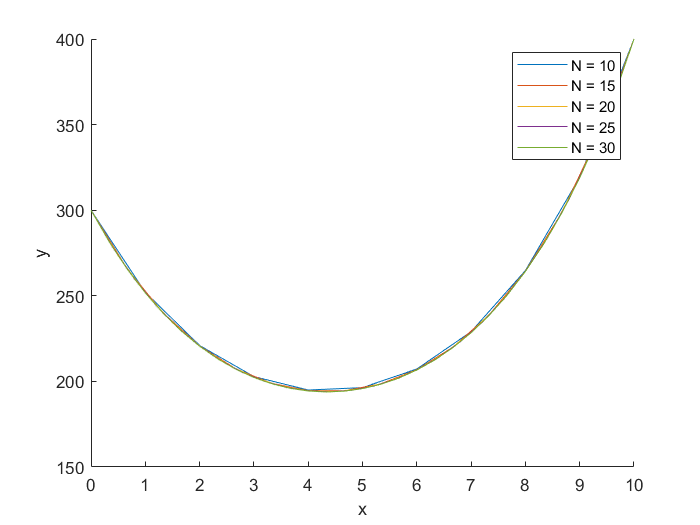
\includegraphics[width=0.4\textwidth]{wc31.png}
            \caption{\ref{problem: 3}数值解图像}
       \end{figure}

       当然我们对非线性项的近似是很粗糙的, 当$T$远离$T_{\infty}$时误差会很明显, 这也是我们的算法需要改进的一部分.
    \end{solution}

    % -------------------- Bibliography --------------------

    % \newpage
    % \bibliography{bibliography}
    % \bibliographystyle{plain}

    % -------------------- Appendix --------------------

    \newpage
    \appendix

    \section{通用函数}

    \subsection{追赶法}

    \lstinputlisting[
        caption=mychase.m,
        style=MATLAB-editor,
        basicstyle=\mlttfamily\scriptsize
    ]{mychase.m}

    \section{求解脚本}

    \subsection{\ref{problem: 1}}

    \lstinputlisting[
        caption=问题一求解脚本: wc2\_1.m,
        label={matlab: 1},
        style=MATLAB-editor,
        basicstyle=\mlttfamily\scriptsize
    ]{wc2_1.m}

    \subsection{\ref{problem: 2}}

    \lstinputlisting[
        caption=问题二求解脚本: wc2\_2.m,
        label={matlab: 2},
        style=MATLAB-editor,
        basicstyle=\mlttfamily\scriptsize
    ]{wc2_2.m}

    \subsection{\ref{problem: 3}}

    \lstinputlisting[
        caption=问题三求解脚本: wc2\_3.m,
        label={matlab: 3},
        style=MATLAB-editor,
        basicstyle=\mlttfamily\scriptsize
    ]{wc2_3.m}

\end{document}
